\documentclass[border=10pt]{standalone}
\usepackage{pgfplots}
\pgfplotsset{compat=1.18}
\begin{document}
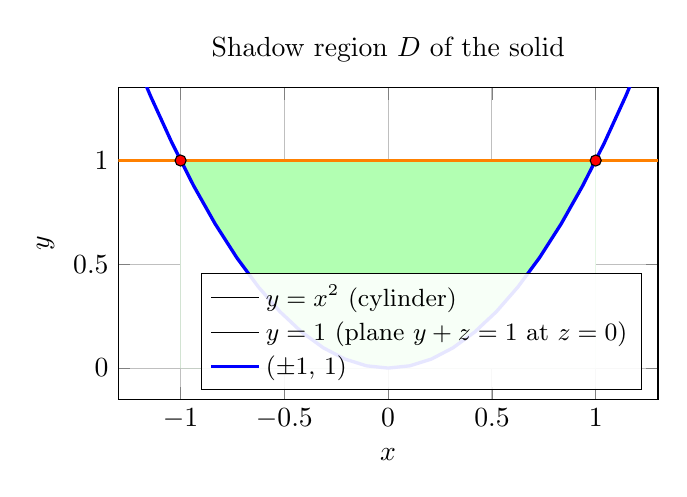
\begin{tikzpicture}
\begin{axis}[
    xlabel={$x$}, ylabel={$y$},
    xmin=-1.3, xmax=1.3, ymin=-0.15, ymax=1.35,
    title={Shadow region $D$ of the solid},
    axis equal image, grid,
    legend pos=south east, legend cell align=left,
    legend style={font=\small, fill=white, fill opacity=0.9, text opacity=1}]
% shaded shadow region between y=x^2 and y=1
\addplot[fill=green!30, draw=none, domain=-1:1] {1} \closedcycle;
\addplot[fill=white, draw=none, domain=-1:1] {x^2} \closedcycle;
% cylinder y = x^2
\addplot[blue, very thick, domain=-1.25:1.25] {x^2};
\addlegendentry{$y=x^2$ (cylinder)}
% line y = 1
\addplot[orange, very thick, domain=-1.3:1.3] {1};
\addlegendentry{$y=1$ (plane $y+z=1$ at $z=0$)}
% intersection points
\addplot[only marks, mark=*, mark options={fill=red, draw=black}] coordinates {(-1,1) (1,1)};
\addlegendentry{$(\pm 1,\,1)$}
\end{axis}
\end{tikzpicture}
\end{document}